%\documentclass{scrartcl}
%\usepackage{beamerarticle}
%%\usepackage{dtsc-beamer}
%\usepackage{fullpage}

\documentclass[9pt]{beamer}
\usetheme{boxes}
\usetheme{Boadilla}
\usecolortheme{beaver}
%\usecolortheme{sidebartab}
% \usefonttheme{structurebold}
\usefonttheme{serif}

%gets rid of bottom navigation bars
\setbeamertemplate{footline}[page number]{}

%gets rid of navigation symbols
\setbeamertemplate{navigation symbols}{}


% \usepackage{helvet}
\usepackage{amsmath, amssymb}
\usepackage{color}
%\usepackage{asymptote}
\usepackage{mathrsfs}
\usepackage{dsfont}
\usepackage{url}
\usepackage{cancel}
\usepackage{tikz}
\usetikzlibrary{fit,positioning}
\usetikzlibrary{shapes,matrix,decorations.markings,arrows}
\usetikzlibrary{graphs}
\usepackage{bbm}
\def\ind{\mathbbm{1}} %Indicator function
%
\definecolor{darkblue}{rgb}{0.0, 0.0, 0.55}
\definecolor{notsodarkblue}{rgb}{0.0, 0.0, 0.7}
\setbeamercolor{title}{fg=darkblue}
\setbeamercolor{frametitle}{fg=darkblue}
\newcommand{\myitem}{\item[$\bullet$]}
\definecolor{darkgreen}{rgb}{0, 0.55, 0}
\definecolor{lgray}{rgb}{0.9,0.9,0.9}

\newcommand{\LABFIG}[1]{\label{fig:#1}}%{\tt [fig:$\text{$#1$}$]}}




\newcommand{\ve}[1]{\boldsymbol{#1}}
\def\X{\ve{X}}
\def\x{\ve{x}}
\def\y{\ve{y}}
\def\m{\ve{m}}
\def\Sig{\ve{\Sigma}}
\def\E{\mathbb{E}}
\def\J{\ve{J}}
\def\h{\ve{h}}

\newcommand{\mc}[1]{\mathcal{#1}}
\def\sX{\mc{X}}
\def\N{\mc{N}}
\newcommand{\mxf}[3]{m^{#3}_{X_{#1}\rightarrow f_{#2}}(x_{#1})}
\newcommand{\mfx}[3]{m^{#3}_{f_{#2}\rightarrow X_{#1}}(x_{#1})}



\newcommand\Def[1]{{\textbf{Definition:}\\\emph{#1}\\\begin{center} ------------------------ \end{center}}}
\newcommand\Prop[1]{{\textbf{\textcolor{red}{Property:}}\\\emph{#1}\\\begin{center} \textcolor{red}{------------------------} \end{center}}}

\newcommand{\noteB}[1]{\textbf{\textcolor{notsodarkblue}{#1}}}

\newcommand{\noteR}[1]{\textbf{\textcolor{darkred}{#1}}}

\newcommand{\noteG}[1]{\textbf{\textcolor{darkgreen}{#1}}}

\newcommand{\snoteB}[1]{{\textcolor{darkblue}{#1}}}

\newcommand{\snoteR}[1]{{\textcolor{darkred}{#1}}}

\newcommand{\snoteG}[1]{{\textcolor{darkgreen}{#1}}}


\newcommand{\fs}[2]{#2}

\title[]{Gaussian BP}
\author[\textcolor{white}{Advanced Digital Communications}]{Introduction to Graphical Models and Inference for Communications\\\vspace*{3mm}{\small \textcolor{black}{UC3M}}
}
%\date[08/02/2016]{{08/02/2016}}
\institute{\textcolor{white}{}}
\AtBeginSection[]
{
  \begin{frame}<beamer>{Index}
    \tableofcontents[currentsection,currentsubsection]
  \end{frame}
}

\begin{document}

\frame{
\titlepage
\thispagestyle{empty}
\begin{center}
\includegraphics[scale=0.05]{Figuras/uc3m-logo.pdf}
\end{center}
}


\frame{
\frametitle{Today}

\begin{itemize}
\item One particular scenario: we want to perform inference over Gaussian probability distributions that factorize according to a graphical model
\item Factor Graphs.
\item Belief Propagation naturally extends to this scenario by replacing summations to integrals (\emph{Gaussian Belief Propagation}).
\item GaBP is exact for Gaussian tree factor graphs.
\item GaBP computes the exact mean for graphs with cycles, but approximated covariance matrix.
\end{itemize}


}

\section{Multivariate Gaussian distribution}


\frame{
\frametitle{Multivariate Gaussian distribution}
Let $\X$ be a Gaussian random vector ($\x\in\mathbb{R}^n$). 
\begin{itemize}
\item \textbf{Covariance form:} the probability density function is 
\begin{align*}
\mu(\x)=\frac{1}{(2\pi)^{n/2}|\Sig|^{1/2}}\exp\left\{-\frac{1}{2}(\x-\m) ^T \Sig^{-1}(\x-\m) \right\}
\end{align*}
denoted as $\x\sim\mathcal{N}(\m,\Sig)$ with mean $\m=\E[\x]$ and covariance matrix $\Sig=\E[(\x-\m)^T(\x-\m)]$.
\item \textbf{Natural form:} the probability density function is 
\begin{align*}
\mu(\x)\propto \exp\left\{ -\frac{1}{2} \x^T \ve{J} \x+\ve{h}^{T}\x\right\}
\end{align*}
denoted as $\x\sim\mathcal{N}^{-1}(\ve{h},\ve{J})$ with potential vector $\h$ and \emph{precision matrix} $\J$.
\item Note $\J=\Sig^{-1}$ and $\h=\J\m$.
\end{itemize}

\begin{block}{}
Gaussian graphical models typically describe Gaussian joint probability density functions in \textbf{natural form}.
\end{block}

}

\frame{
\frametitle{Product of two Gaussians}

\begin{align*}
&\mathcal{N}(\m_a,\Sig_a)\mathcal{N}(\m_b,\Sig_b)\\
=&\mathcal{N}^{-1}(\ve{h}_a,\ve{J}_a)\mathcal{N}^{-1}(\ve{h}_b,\ve{J}_b)\\
=&\mathcal{N}^{-1}(\ve{h}_a+\h_b,\ve{J}_a+\J_b)=\N(\m,\Sig)
\end{align*}
where
\begin{align*}
\Sig=\left(\ve{J}_a+\J_b\right)^{-1}\qquad \m=\Sig(\ve{h}_a+\h_b)
\end{align*}




}

\frame{
\frametitle{Marginalization via algebraic manipulation}
\begin{itemize}
\item Let $\y=\ve{A} \x+ \ve{v}$, where $\x\sim\mathcal{N}(\m_x,\Sig_x)=\mathcal{N}^{-1}(\h_x,\J_x)$ and $\ve{v}\sim\mathcal{N}(\m_v,\Sig_v)=\mathcal{N}^{-1}(\h_v,\J_v)$, then
\begin{align*}
\mu(\y)&=\int_{-\infty}^{\infty}\mu(\y|\x)\mu(\x)d\x?
\end{align*}
\end{itemize}

\begin{align*}
\mu(\y|\x)\mu(\x)\propto &\exp\Big\{\frac{-1}{2}\y^T \J_v \y+(\J_v\m_v)^T\y +(\J_v\ve{A}\x)^T\y-\frac{-1}{2}\x^T \J_x \x+(\J_x\m_x)^T\x \Big\}\\
\propto&\Big\{ \frac{-1}{2} \left[\begin{array}{c}\y \\ \x \end{array} \right]^T \J_* \left[\begin{array}{c}\y \\ \x \end{array} \right] +†\h^T_* \left[\begin{array}{c}\y \\ \x \end{array} \right]  \Big\}
\end{align*}
where
\begin{align*}
\J_*=\left[\begin{array}{cc} \J_v & -\J_v\ve{A} \\ -(\J_v\ve{A})^T & \J_x \end{array}\right] \qquad \h_*=\left[\begin{array}{c}\h_v \\ \h_x \end{array}\right]
\end{align*}

}

\frame{
\begin{align*}
\J_*=\left[\begin{array}{cc} \J_x & -\J_v\ve{A} \\ -(\J_v\ve{A})^T & \J_v \end{array}\right] \qquad \h_*=\left[\begin{array}{c}\h_v \\ \h_x \end{array}\right]
\end{align*}

Marginalization its easy if we obtain the covariance form of the joint distribution. Applying the matrix inversion lemma:
\begin{align*}
\left[\begin{array}{cc} \J_v & -\J_v\ve{A} \\ -(\J_v\ve{A})^T & \J_x \end{array}\right]^{-1}=
\left[\begin{array}{cc} 
\ve{S}^{-1} & \ve{S}^{-1}\J_v\ve{A}\J^{-1}_x \\  \J^{-1}_x(\J_v\ve{A})^T\ve{S}^{-1} & \J^{-1}_x+\J^{-1}_x(\J_v\ve{A})^T\ve{S}^{-1} \J_v\ve{A}\J^{-1}_x
\end{array}\right]
\end{align*}
where $\ve{S}=\J_v-\J_v\ve{A}\J_x^{-1}(\J_v\ve{A})^T$.

\begin{block}{Therefore}
\begin{align*}
p(\y)=\mathcal{N}^{-1}(\h_y,\J_y) 
\end{align*}
where
\begin{align*}
 \J_y=\J_v-\J_v\ve{A}\Sig_x\ve{A}^T\J_v^T \qquad \h_y=\h_v+\J_v\ve{A}\Sig_x\h_x
\end{align*}
\end{block}

}

\section{Gaussian BP over a particular example}

\frame{
Let $X_i\in\sX$ $i=1,\ldots,5$ be a collection of real R.V.  with joint distribution of the form
\begin{align*}
\mu(\x)=\frac{1}{Z}f_1(x_1,x_2)f_2(x_2,x_3)f_3(x_2,x_4)f_4(x_4,x_5)\prod_{i=1}^{5}g(x_i)
\end{align*}
where
\begin{align*}
f_1(x_1,x_2)=\exp\{F_{1}x_1x_2\} \qquad f_2(x_2,x_3)=\exp\{F_{2}x_2x_3\}\\
f_3(x_2,x_4)=\exp\{F_{3}x_2x_4\} \qquad f_4(x_4,x_5)=\exp\{F_{4}x_4x_5\}
\end{align*}
 and 
\begin{align*}
g(x_i)=\exp\{b_i x_i-\frac{1}{2}\pi_i x_i^2\}
\end{align*}

\begin{figure}
\begin{tabular}{c}
\includegraphics[scale=0.5]{Figuras/Graph_1.pdf}
\end{tabular}
\end{figure}
%
%\begin{block}{Assume we want to compute}
%\begin{align*}
%P(x_1)=\sum_{\x\sim x_1}P(x_1,x_2,x_3,x_4,x_5)
%\end{align*}
%\textbf{\textcolor{red}{By brute force... $|\sX|^{5}$ sums.}} 
%\end{block}
%
%


}

\frame{
\begin{itemize}
\item $\mu(\x)$ is a Gaussian distribution defined in natural form!
\end{itemize}
\begin{align*}
\J&=\left[\begin{array}{ccccc}
\pi_1 & -F_{1} & 0 & 0 & 0 \\
-F_{1} & \pi_2 & -F_{2} & -F_{3} & 0\\
0 & -F_{2} & \pi_3 & 0 & 0 \\
0 &  -F_{3} & 0 & \pi_4 & -F_{4}  \\
0 & 0 & 0 & -F_{4} &  \pi_5
\end{array}
\right]\\\\
\h&=\left[\begin{array}{ccccc}
b_1 & b_2 & b_3 & b_4 & b_5
\end{array}
\right]^T
\end{align*}

\begin{block}{}
Computing the mean $\m$ and covariance matrix $\Sig$ requires computing $\Sig=\J^{-1}$ and $\m = \J^{-1} \h$. $O(n^3)$ cost! 
\end{block}

\begin{exampleblock}{}
BP provides a way to exploit graph structure to perform this
computation in $\mathcal{O}(n)$ time instead of $O(n^3)$. It is only exact when the graph is a tree!
\end{exampleblock}

\begin{alertblock}{}
If the Gaussian graphical model has cycles, GBP still computes the exact $\m$, but only an estimation to $\Sig$.
\end{alertblock}

}

%\section{Gaussian BP}


\frame{
\frametitle{Gaussian BP algorithm}

\begin{itemize}
\item It is described as a \emph{message-passing algorithm}.
\item Messages represent \emph{local computations} at each node of the graph.
\item The FG has leave factors (only connected to one variable) and pairwise factors (connected to two variables).
\item Integrals instead of sums. The rest of the algorithm remains unaltered.
\end{itemize}

\begin{figure}
\begin{tabular}{c}
\includegraphics[scale=0.5]{Figuras/Graph_4.pdf}
\end{tabular}
\end{figure}

}

\frame{
\frametitle{Iteration 0}
\begin{itemize}
\item Messages send by variable nodes are initialized by their  leave factors
\end{itemize}
E.g.
\begin{align*}
m^{0}_{x_2\rightarrow f_2}(x_2)=g(x_2)=\exp\{b_2 x_2-\frac{1}{2}\pi_2 x_2^2\}\sim \mathcal{N}^{-1}(b_2,\pi_2) \quad   \text{\color{blue}{Gaussian message!}}
\end{align*}
\begin{itemize}
\item Messages send by the $f_j$ factors are computed as usual but replacing sums by integrals.
\end{itemize}
E.g.
\begin{align*}
m^{0}_{f_1\rightarrow x_1}(x_1)&=\int \exp\{F_{1}x_1x_2\}\exp\{b_2 x_2-\frac{1}{2}\pi_2 x_2^2\}  dx_2\\
&=\int \exp\Big\{-\frac{1}{2} \left[\begin{array}{c} x_1 \\ x_2 \end{array}\right]^T \left[\begin{array}{cc} 0 & -F_1 \\ -F_1 & \pi_2\end{array} \right] \left[\begin{array}{c} x_1 \\ x_2 \end{array}\right]+\left[\begin{array}{c} 0 \\b_2 \end{array}\right]^T\left[\begin{array}{c} x_1 \\ x_2 \end{array}\right]\Big\} dx_2\\
&\sim \mathcal{N}^{-1}(F_1\pi_2^{-1}b_2,F_1^2\pi_2^{-1})=\mathcal{N}^{-1}(h^{0}_{f_1\rightarrow x_1}, J^{0}_{f_1\rightarrow x_1})\quad \text{\color{blue}{Gaussian message!}}
\end{align*}
}

\frame{
\frametitle{At iteration $\ell$}

\begin{itemize}
\item \textbf{Step 1:} Variable nodes multiply their incoming messages to send a new message to factors.
\end{itemize}
E.g.
\begin{align*}
m^{\ell}_{x_2\rightarrow f_3}(x_2)&=\mathcal{N}^{-1}(h^{\ell-1}_{f_1\rightarrow x_2}, J^{\ell-1}_{f_1\rightarrow x_2})\mathcal{N}^{-1}(h^{\ell-1}_{f_2\rightarrow x_2}, J^{\ell-1}_{f_2\rightarrow x_2})\\
&=\mathcal{N}^{-1}(h^{\ell-1}_{f_1\rightarrow x_2}+h^{\ell-1}_{f_2\rightarrow x_2}, J^{\ell-1}_{f_1\rightarrow x_2}+J^{\ell-1}_{f_2\rightarrow x_2})\\
&=\mathcal{N}^{-1}(h^{\ell}_{x_2\rightarrow f_3}, J^{\ell}_{x_2\rightarrow f_3}).
\end{align*}
}


\frame{
\frametitle{At iteration $\ell$}
\begin{itemize}
\item \textbf{Step 2:} Factor nodes compute the messages to variable nodes by marginalization.
\end{itemize}
E.g.
\begin{align*}
&m^{\ell}_{f_3\rightarrow x_4}(x_4)=\int \exp\{F_{3}x_2x_4\}\mathcal{N}^{-1}(h^{\ell}_{x_2\rightarrow f_3}, J^{\ell}_{x_2\rightarrow f_3})  dx_2\\
&=\int \exp\Big\{-\frac{1}{2} \left[\begin{array}{c} x_2 \\ x_4 \end{array}\right]^T \left[\begin{array}{cc} 0 & -F_3 \\ -F_3 & J^{\ell}_{x_2\rightarrow f_3}\end{array} \right] \left[\begin{array}{c} x_2 \\ x_4 \end{array}\right]+\left[\begin{array}{c} 0 \\h^{\ell}_{x_2\rightarrow f_3} \end{array}\right]^T\left[\begin{array}{c} x_2 \\ x_4 \end{array}\right]\Big\} dx_2\\
&\sim \mathcal{N}^{-1}(\frac{F_3 h^{\ell}_{x_2\rightarrow f_3}}{J^{\ell}_{x_2\rightarrow f_3}},\frac{F_3^2}{J^{\ell}_{x_2\rightarrow f_3}})=\mathcal{N}^{-1}(h^{\ell}_{f_3\rightarrow x_4}, J^{\ell}_{f_3\rightarrow x_4})\quad \text{\color{blue}{Gaussian message!}}
\end{align*}

\begin{block}{}
All messages are Gaussian! The parameters of the Gaussian messages are computed in closed form without doing any integral! 
\end{block}

\begin{exampleblock}{}
Convergence is guaranteed and achieved in a finite number  $\ell_*$ of iterations. The overall complexity is $\mathcal{O}(\ell_*n)$.
\end{exampleblock}
}

\section{Gaussian Hidden Markov Models}

\frame{
\frametitle{Gaussian Hidden Markov Models}

\begin{block}{}
\begin{itemize}
\item Wireless communication channels.
\item Speech processing.
\item Tracking applications.
\end{itemize}
\end{block}

\begin{figure}
\begin{tabular}{c}
\includegraphics[scale=0.75]{Figuras/HMM.pdf}
\end{tabular}
\end{figure}



}

\frame{
\frametitle{Gaussian Hidden Markov Models}
\begin{itemize}
\item States $\x_t\in\mathbb{R}^{d}$.
\item State transition matrix $\ve{A}\in\mathbb{R}^{d\times d}$.
\item Process noise $\ve{v}_t\in\mathbb{R}^{p}$ and $\sim\mathcal{N}(\ve{0},\Sig_v)$ for some $\Sig_v\in\mathbb{R}^{p\times p}$.
\item Dynamic equations:
\begin{align*}
\x_{t+1}=\ve{A}\x_t+\ve{B}\ve{v}_t\\
\x_0\sim \mathcal{N}(0,\Sig^{0}_{x})
\end{align*}
\end{itemize}

\begin{itemize}
\item Noisy observation  $\y_t\in\mathbb{R}^{d'}$:
\begin{align*}
\y_t=\ve{C}\x_t+\ve{w}_t
\end{align*}
where $\ve{C}\in\mathbb{R}^{d'\times d}$ and $\ve{w}_t\sim\mathcal{N}(0,\Sig_w)$.
\end{itemize}

\begin{figure}
\begin{tabular}{c}
\includegraphics[scale=0.6]{Figuras/HMM.pdf}
\end{tabular}
\end{figure}

}

\frame{
\frametitle{Gaussian Hidden Markov Models}
\begin{itemize}
\item In summary, for $\Sig_h=\ve{B}\Sig_v\ve{B}^T$ we have
\begin{align*}
\x_0&\sim \mathcal{N}(0,\Sig^{0}_{x})\\
\x_{t+1}|\x_t &\sim \mathcal{N}(\ve{A}\x_t,\Sig_h)\\
\y_t|\x_t &\sim \mathcal{N}(\ve{C}\x_t, \Sig_w)
\end{align*}
\item Factorization
\begin{align*}
\mu(\x,\y)=\mu(x_0)\mu(\y_0|x_0)\mu(\x_1|\x_0)\mu(\y_1|x_1)\mu(\x_2|\x_1)\mu(\y_2|x_2)\ldots
\end{align*}
\item Gaussian graphical model with no cycles!! GaBP is exact and cheap!
\item This factorization can be expanded as the product of leave factors and pairwise factors.
\end{itemize}



}

\frame{
\frametitle{Inference over Gaussian HMMs}

\begin{block}{Forward/Backward algorithm}
Given $\y_0,\y_2,\ldots,\y_L$, use GaBP to compute the (Gaussian) marginal for each state $\x_1,\x_2,\ldots,\x_L$.
\end{block}

\begin{block}{Kalman filter}
Given the actual observation $\y_t$ and the observations in the past $\y_0,\y_2,\ldots,\y_t-1$, use GaBP to compute the mean of $\x_t$, $\mathbb{E}[\x_t]$.
\end{block}


}

\section{Extension to any distribution?}

\frame{
\frametitle{BP over any graphical models}
\begin{itemize}
\item So far, we have applied BP to discrete and Gaussian graphical models. 
\item In the Gaussian case, we can avoid integration by algebraic manipulation.
\item The same update rules can be applied to any Graphical model. However, integrals of the form 
\begin{align*}
\int_{\x_j\sim x_i} f_j(\x_j) \prod_{u\in\N(f_j)}\m_{x_u\rightarrow f_j}(x_u) d(\x_j\sim x_i)
\end{align*}
are intractable in general! we cannot solve the integrals!!
\end{itemize}




}

\frame{
\begin{block}{Approximate message passing (APM)}
Approximate BP messages by Gaussian distributions:
\begin{itemize}
\item Compressed sensing \url{http://people.ee.duke.edu/~lcarin/AMP1.pdf}
\item Efficient multiuser detection in CDMA systems \url{http://arxiv.org/pdf/0810.1729.pdf}
\item Communications over Fading ISI channels:
\url{http://ieeexplore.ieee.org/stamp/stamp.jsp?arnumber=04907469}
\item $\ldots$
\end{itemize}
\end{block}

\begin{exampleblock}{Alternatives}
Instead of approximating the BP messages, construct directly a tractable Gaussian approximation to the joint pdf.
\begin{itemize}
\item Variational Inference and Mean Field.
\item Expectation Propagation.
\end{itemize}
\end{exampleblock}



}

\end{document}

